\documentclass[11pt]{amsart}
\usepackage{geometry}                % See geometry.pdf to learn the layout options. There are lots.
\geometry{letterpaper}                   % ... or a4paper or a5paper or ... 
%\geometry{landscape}                % Activate for for rotated page geometry
%\usepackage[parfill]{parskip}    % Activate to begin paragraphs with an empty line rather than an indent
\usepackage{graphicx}
\usepackage{amssymb}
\usepackage{epstopdf}
\DeclareGraphicsRule{.tif}{png}{.png}{`convert #1 `dirname #1`/`basename #1 .tif`.png}

\title{General description}
\author{Pooth}
%\date{}                                           % Activate to display a given date or no date

\begin{document}
\maketitle
\section{Abstract .... to be written at the end ....}
Triggering on high $p_t$ muons at the projected high luminosity LHC (HL-LHC) with an expected instantaneous luminosity of $10^{35}/(\mathrm{cm}^2 \cdot\mathrm{s})$ will be 
one major challenge for the CMS experiment from 2023 on. With the {\bf M}uon  {\bf T}rack fast {\bf T}ag (MTT) a new detector subsystem is proposed that can help to keep the 
Level-1 trigger rate low enough without increasing the $p_t$ thresholds for single muons. The trigger concept must be extended by combining the information of the inner tracking
system with a fast muon tag which is also able to reduce the problem with ambiguities of simultaneously traversing muons leading to so-called ghost hits in the muon systems. 

\section{Motivation for a Muon Track fast Tag (MTT) at CMS}

From the year 2023 the CMS experiment at the LHC is expected to operate at the high luminosity LHC (HL-LHC). Up to 1000~fb$^{-1}$ of data will be collected per year with an 
instantaneous luminosity that will be increased by a factor of ten compared to the running LHC with a design luminosity of $10^{34}/(\mathrm{cm}^2 \cdot\mathrm{s})$. New physics 
scenarios and extended limits which are expected and hoped for in the coming years are displayed in Figure~\ref{fig:schedule_concept} where the integrated luminosity is shown versus 
time. Various scenarios are under discussion to increase the amount of data to search for events with extremely small cross sections, e.g. increasing beam energy, higher bunch 
crossing frequency and higher number of protons per bunch. The CMS roadmap for the future long shutdowns in shown in Figure~\ref{fig:upgrade_planning}.

To trigger on high $p_t$ muons at $10^{35}/(\mathrm{cm}^2 \cdot\mathrm{s})$ while keeping the Level-1 trigger rate low the trigger concept needs to be extended. With the MTT (see 
Figure~\ref{fig:schedule_concept}, right), a fast 2D trigger system located between the CMS solenoid and the inner muon stations is proposed in~(REFREF) to cope with high 
muon rates without increasing the $p_t$ thresholds. Just increasing the threshold would be an inefficient way as shown in Figure~\ref{fig:pt_threshold}, mainly due to poorly 
reconstructed muon $p_t$ on Level-1. 
\begin{figure}[htbp]
\centering
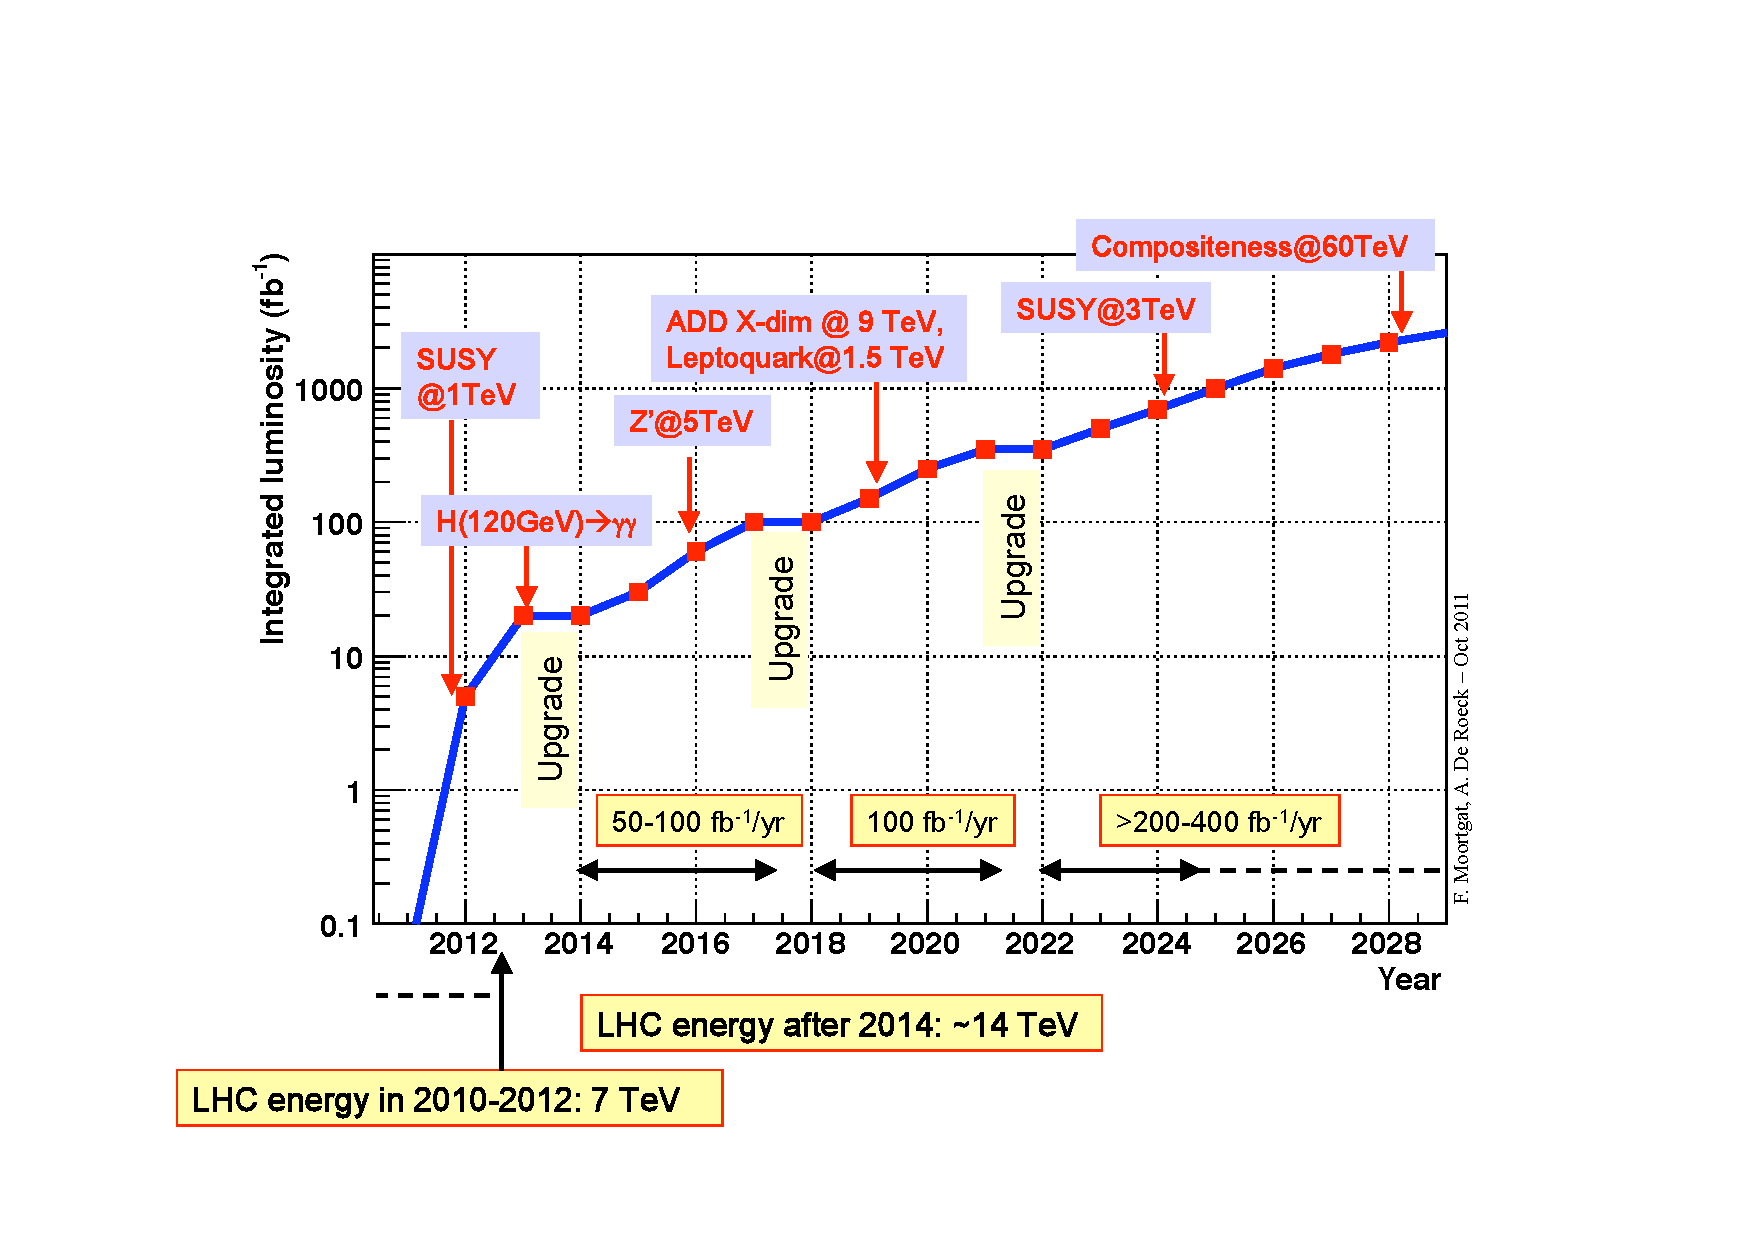
\includegraphics[width=0.45\textwidth]{Figures/pooth/schedule.pdf}
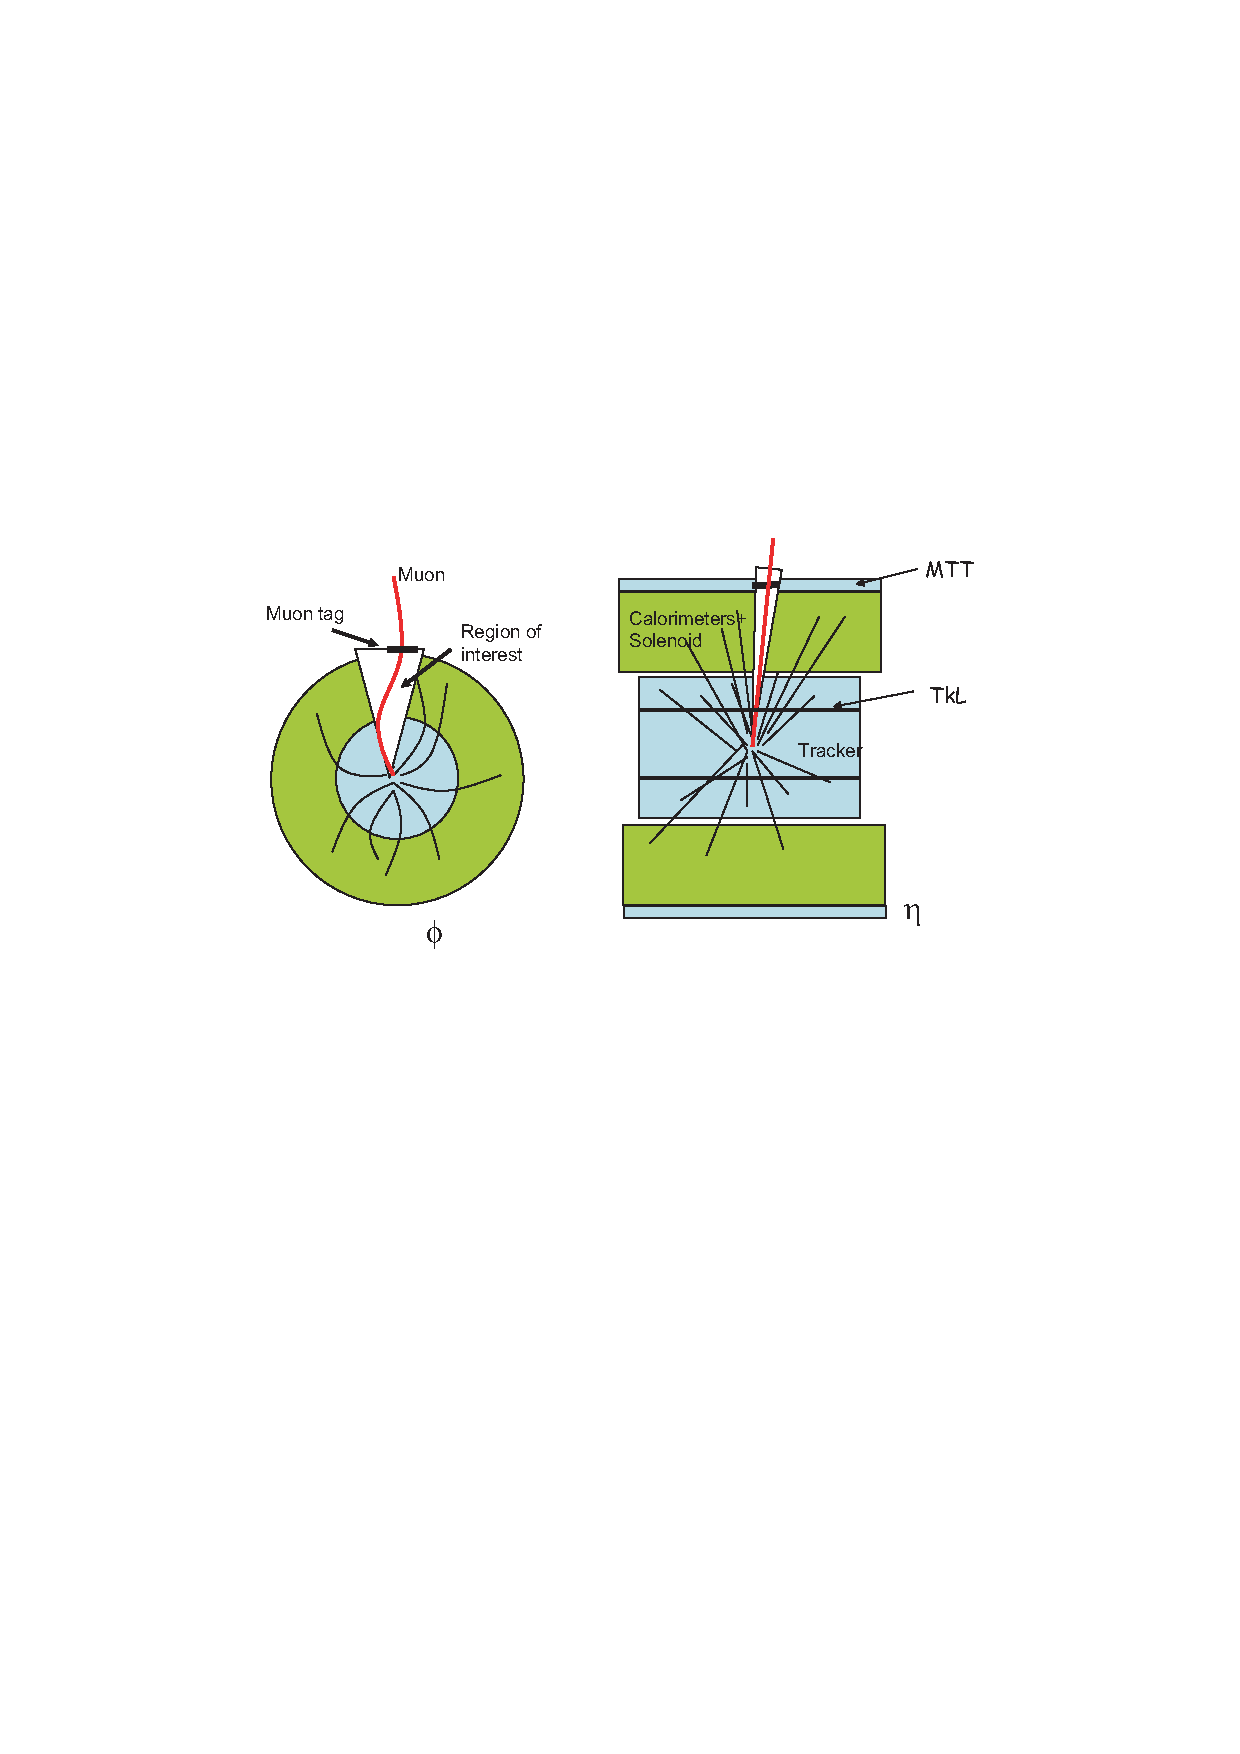
\includegraphics[width=0.52\textwidth]{Figures/pooth/mtt_concept_a.pdf}
\caption{Left: The integrated luminosity versus time for the periods before, between and after the three long shutdowns to come~(REFREF). Right: The Muon Track fast Tag concept~(REFREF) } 
\label{fig:schedule_concept}
\end{figure}

Tiles of fast plastic scintillator material read out by silicon photomultipliers (SiPMs) are under investigation to provide the additional detector layer in the very limited space available 
between the CMS solenoid and the first muon stations. The existing outer layers of the Hadron Calorimeter (HO)  can serve as a perfect testbed for this studies. In the barrel region the 
SiPM signals of the outer layers of the Hadron Outer Calorimeter could be used in the muon trigger at Level-1. The benefits of this layer for MIP identification, punch through rejection 
and resolution of ambiguities in the DT system are described in this note. For Run II a trigger link has been established that makes the HO signals available for building Level-1 muon 
trigger primitives together with inputs from DT and RPC. Based on these data, optimization of the HO granularity for Level-1 muon triggering purposes in Phase-2 can be envisaged. 

By combining the information from various subsystems the muon momentum resolution can be improved in the Level-1 trigger system. The inner silicon based tracking system provides 
an excellent $p_t$ measurement and with the MTT it is possible to define regions of interest for the tracker in case of high $p_t$ muons. In addition the MTT can resolve possible muon 
ambiguities at very high luminosities (ghost rejection). A measured ghost and a possible solution to resolve it are shown in Figure~\ref{fig:ghosts}.
\begin{figure}[htbp]
\centering
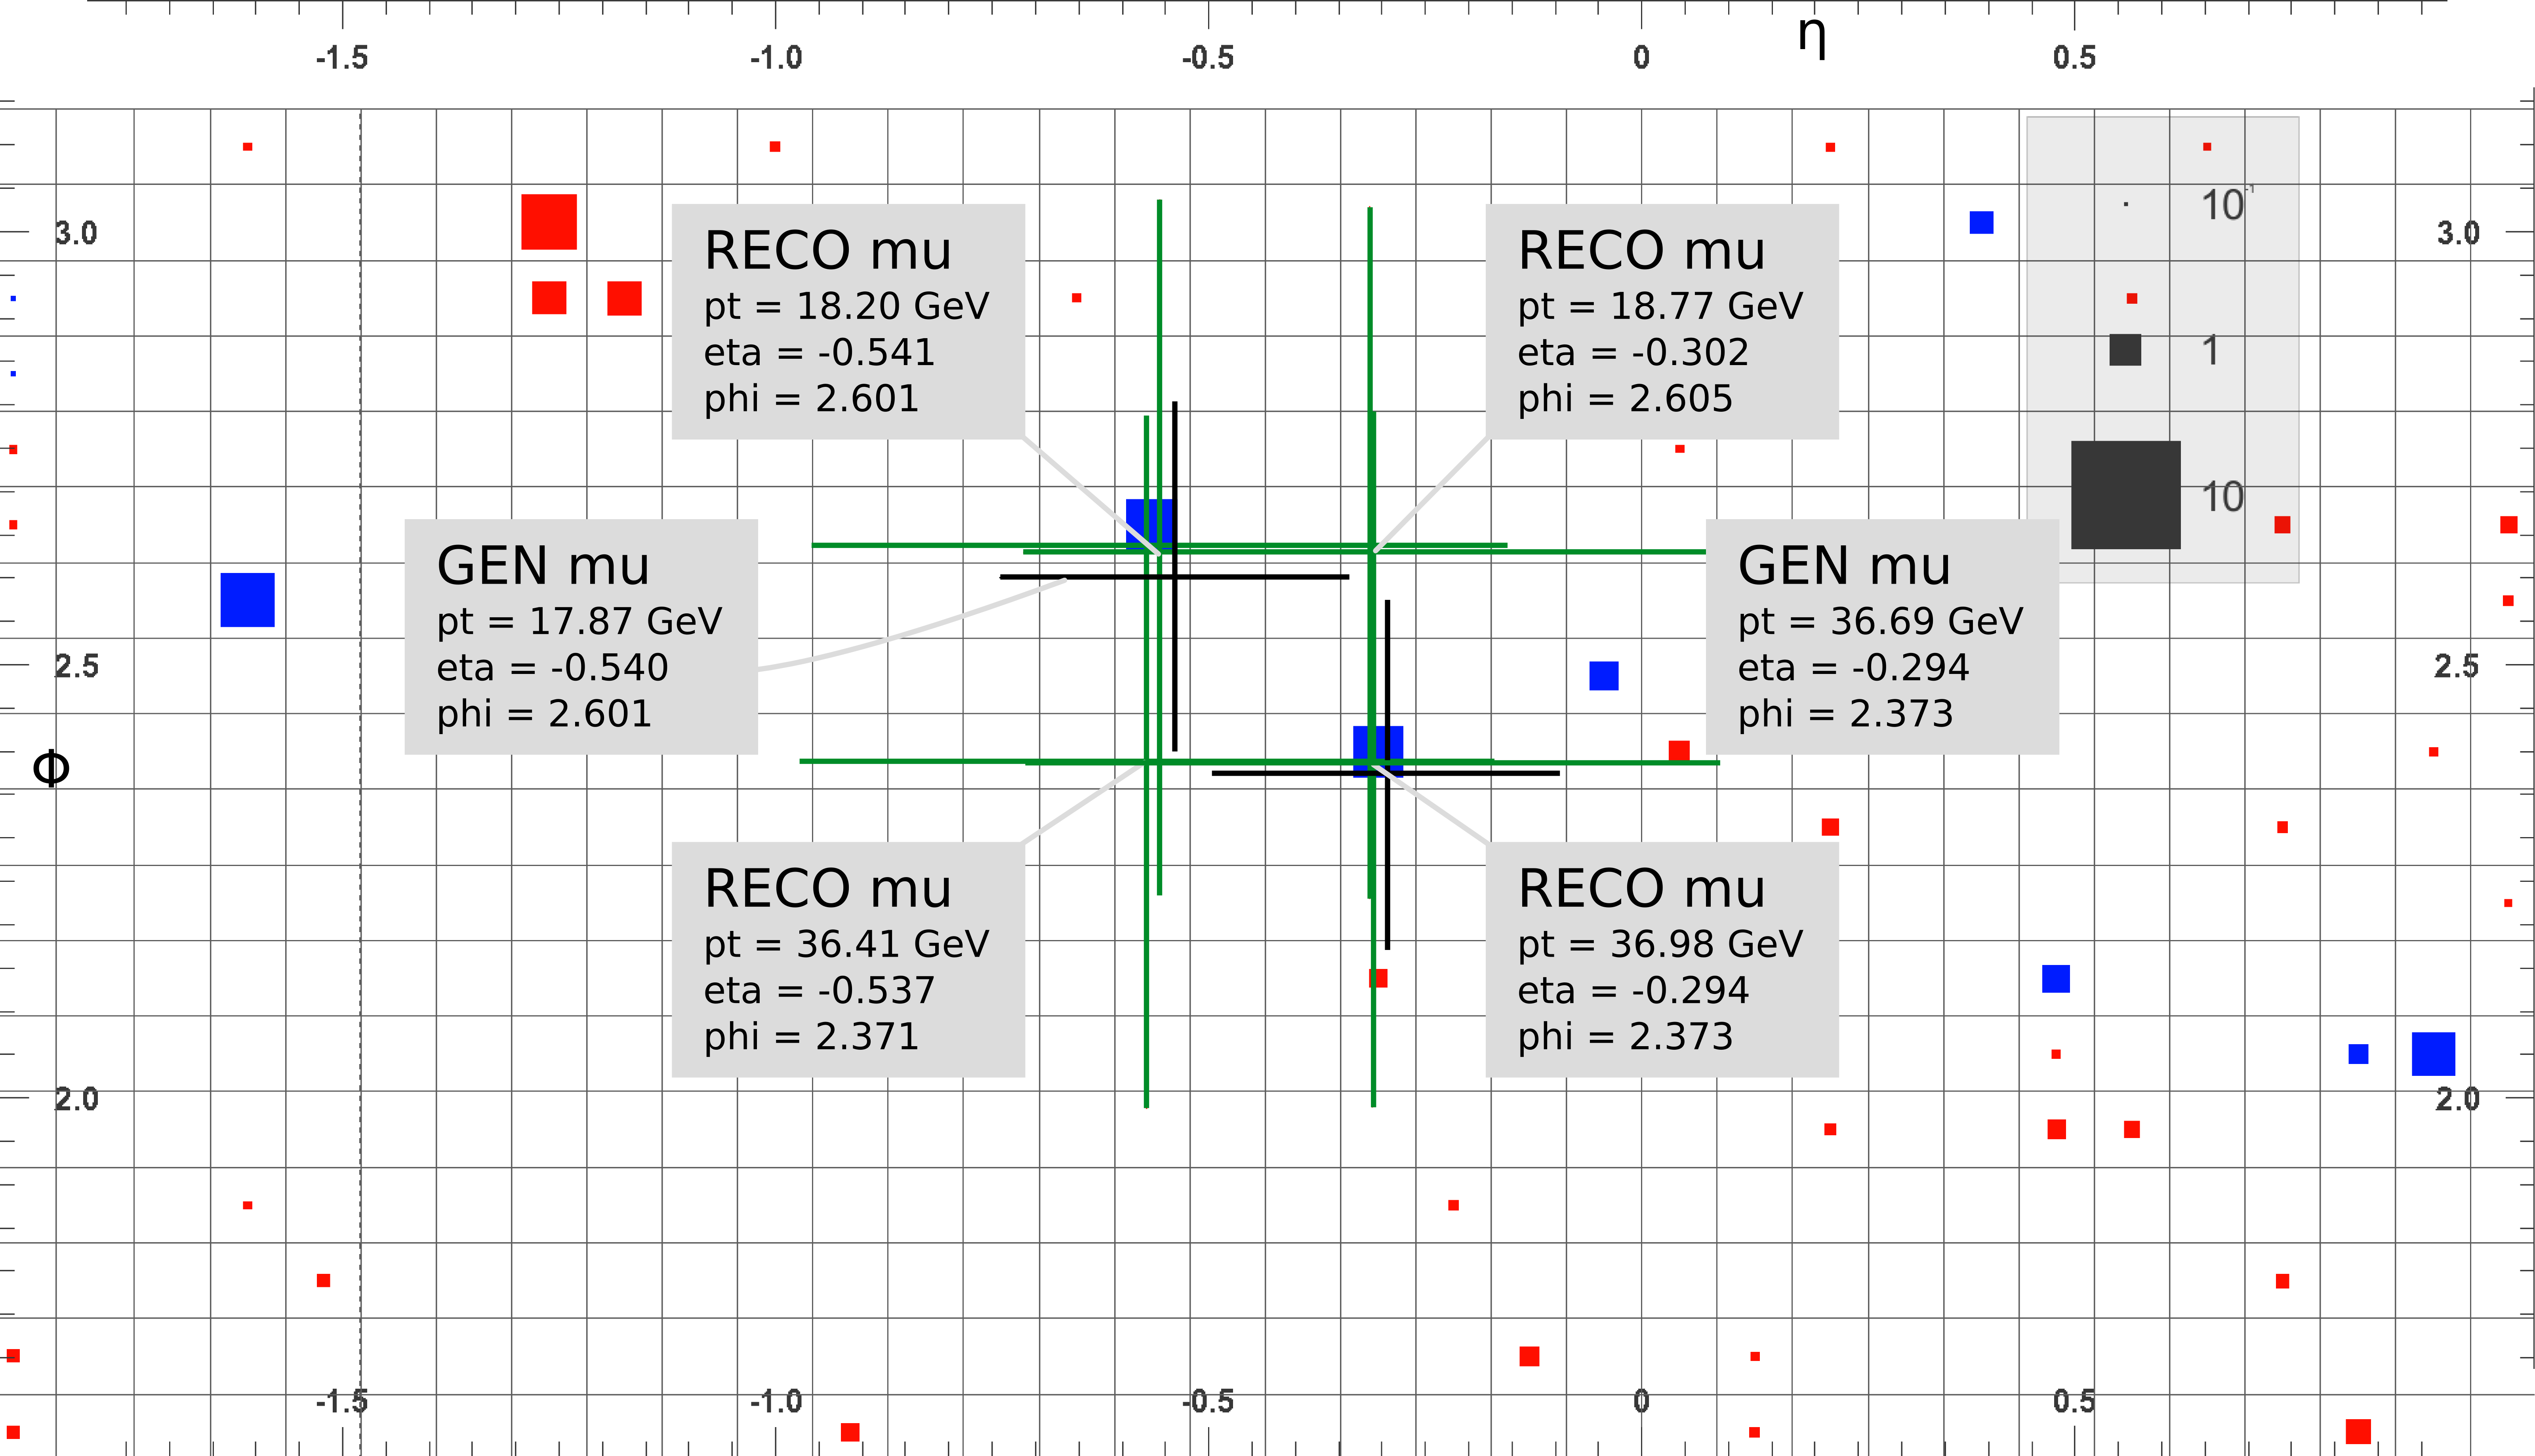
\includegraphics[width=\textwidth]{Figures/pooth/GhostEvent01.png}
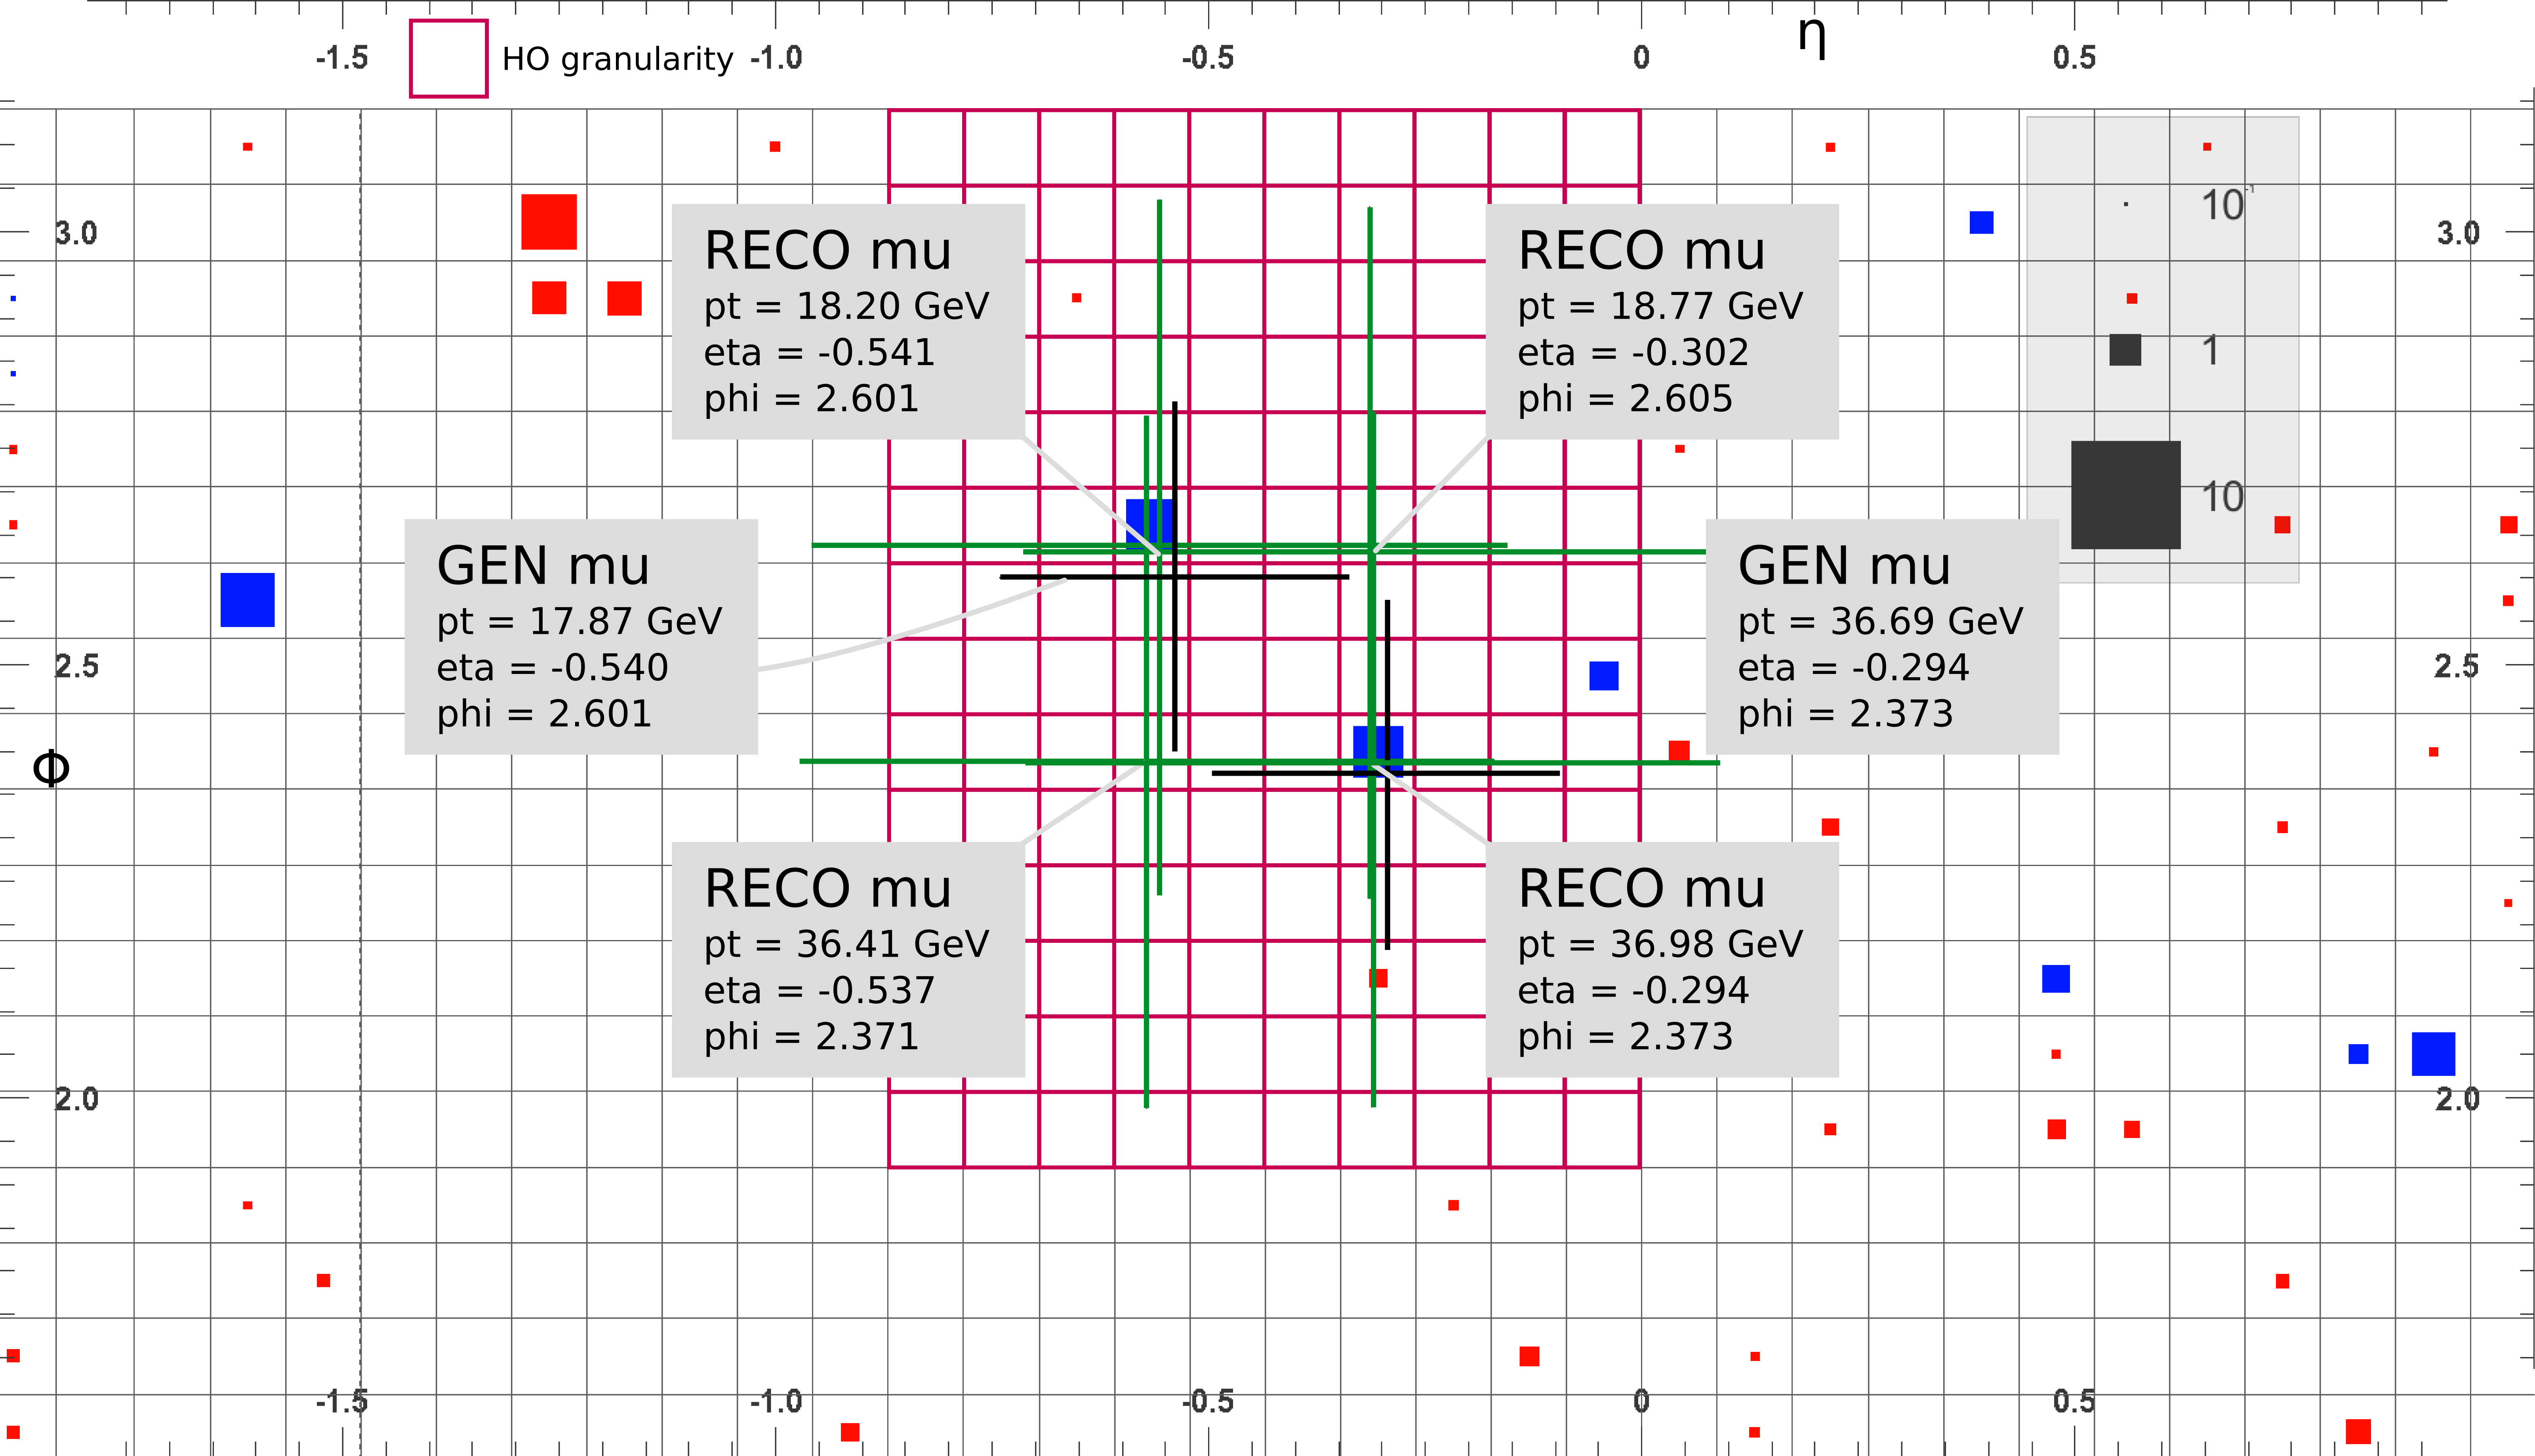
\includegraphics[width=\textwidth]{Figures/pooth/GhostEvent02.png}
\caption{Top: Four reconstructed muons (RECO mu, green crosses) with only two generated muons in the detector (GEN mu, black crosses). 
Bottom: The same event and in addition the HO system overlaid (individual HO tiles shown as pink boxes).} 
\label{fig:ghosts}
\end{figure}
\begin{figure}[htbp]
\centering
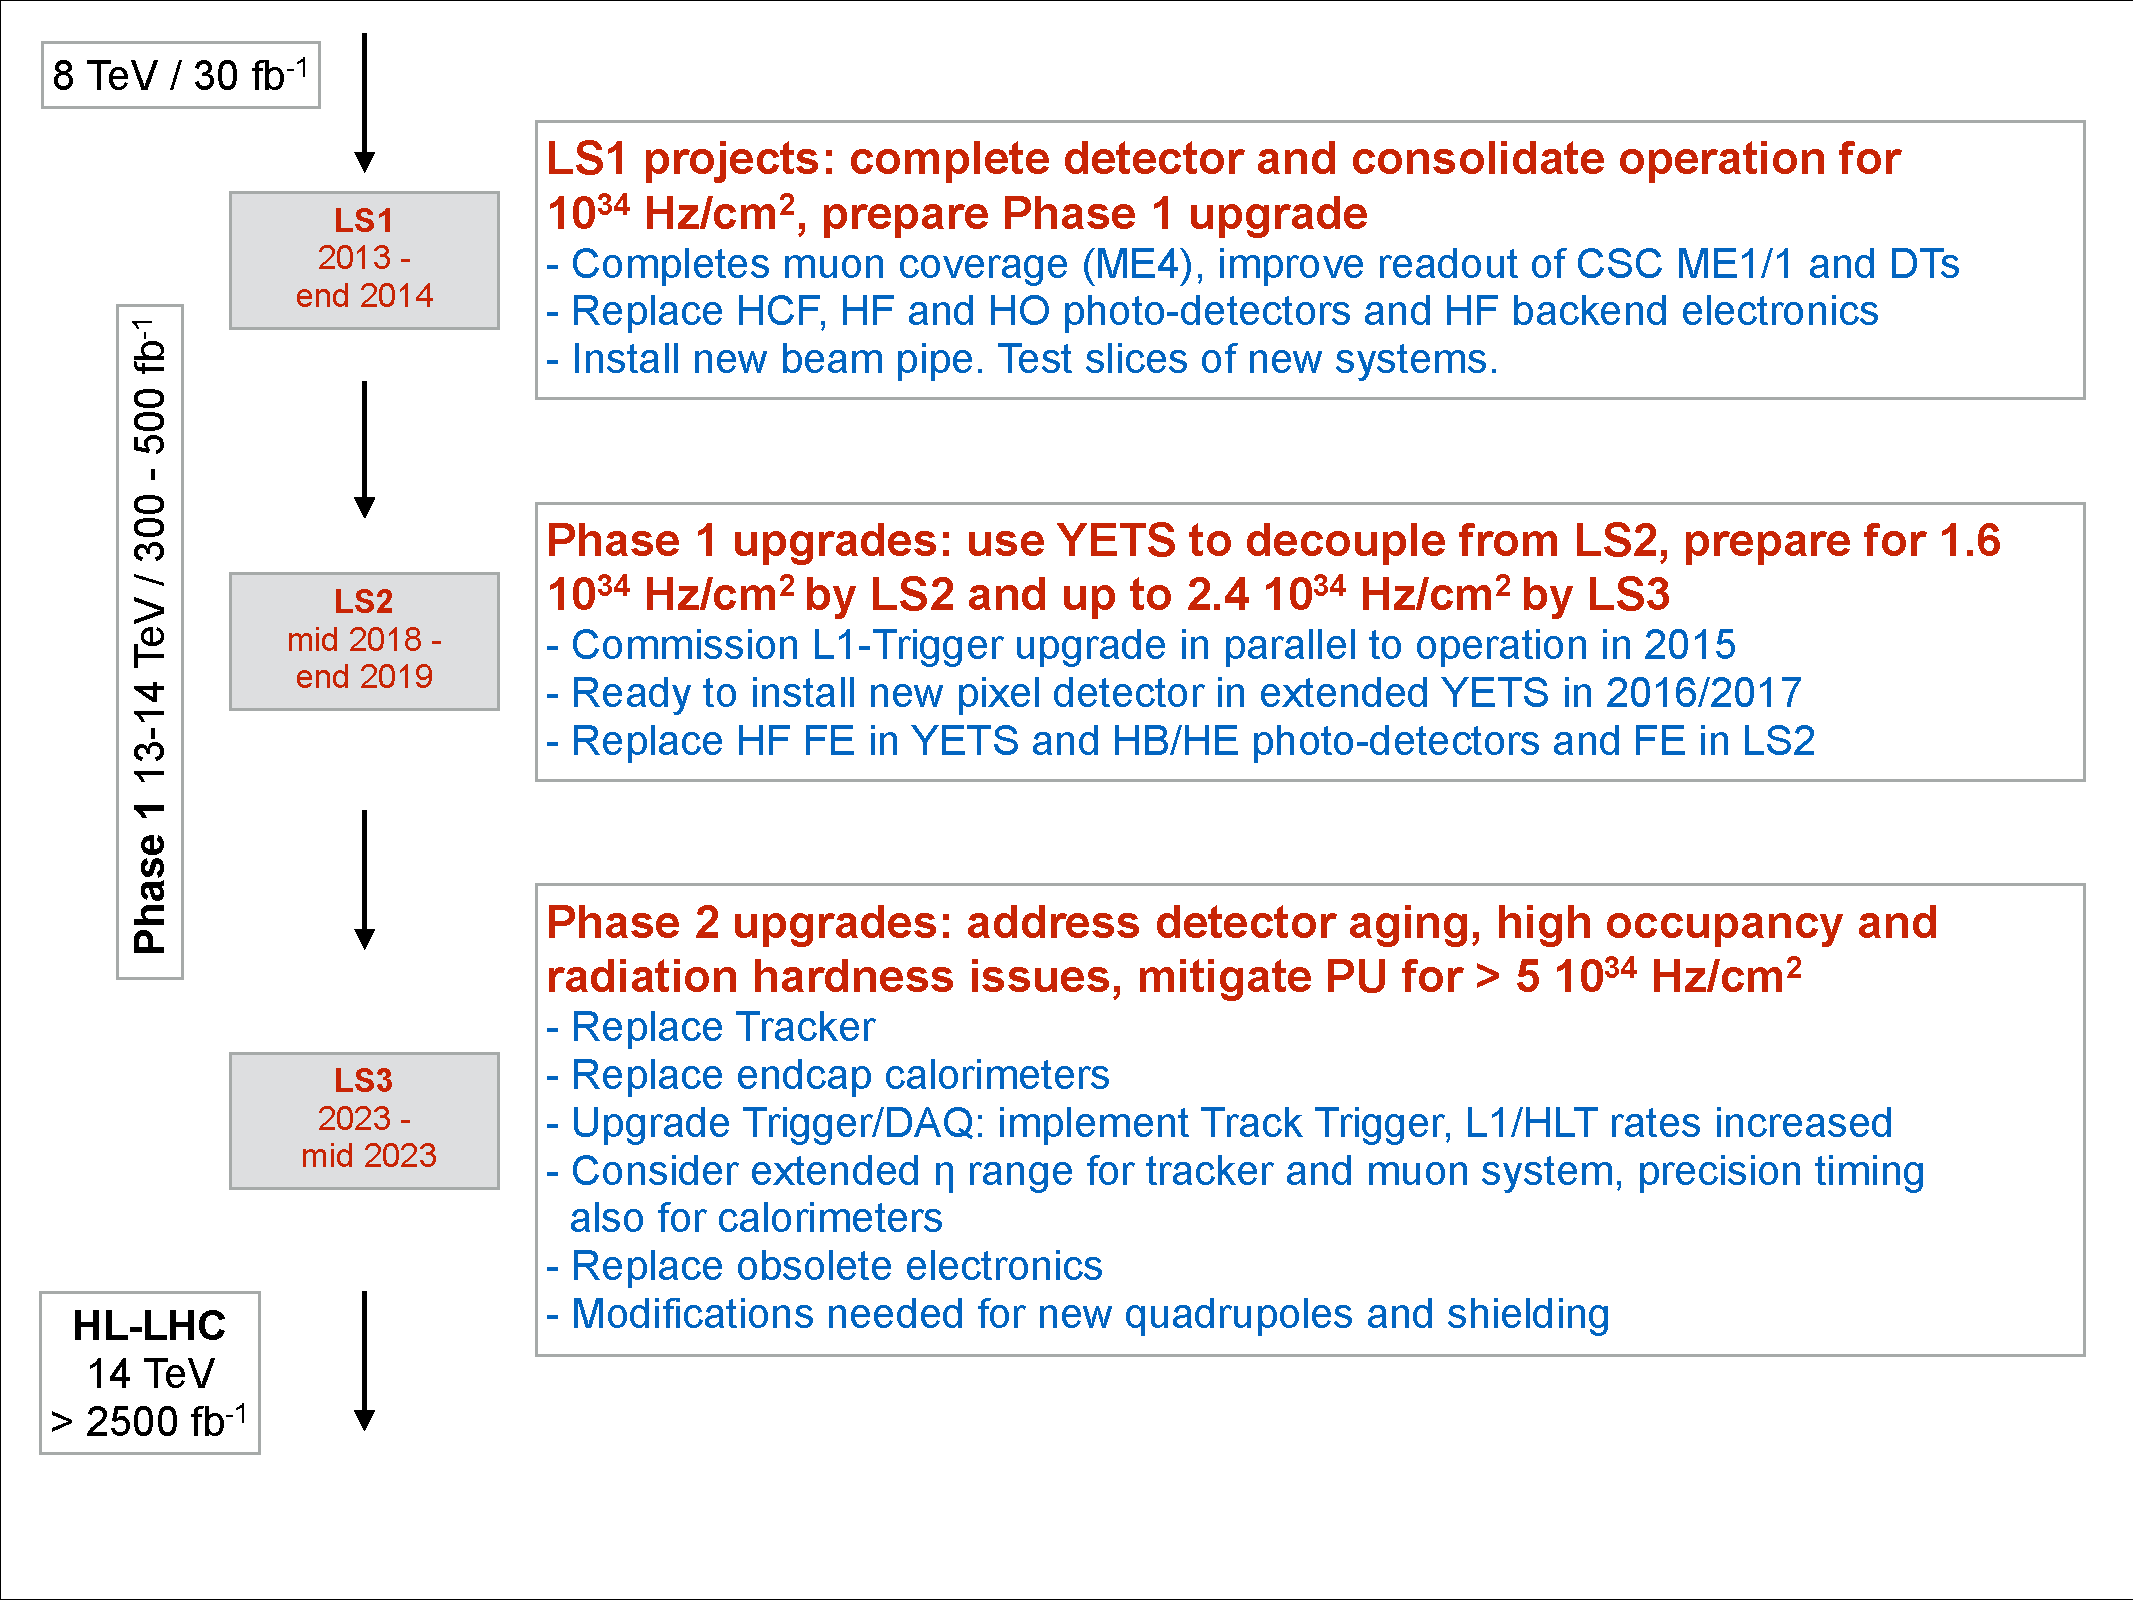
\includegraphics[width=0.8\textwidth]{Figures/pooth/upgrade_planning.pdf}\\
\caption{Upgrade planning~(REFREF).} 
\label{fig:upgrade_planning}
\end{figure}
\begin{figure}[htbp]
\centering
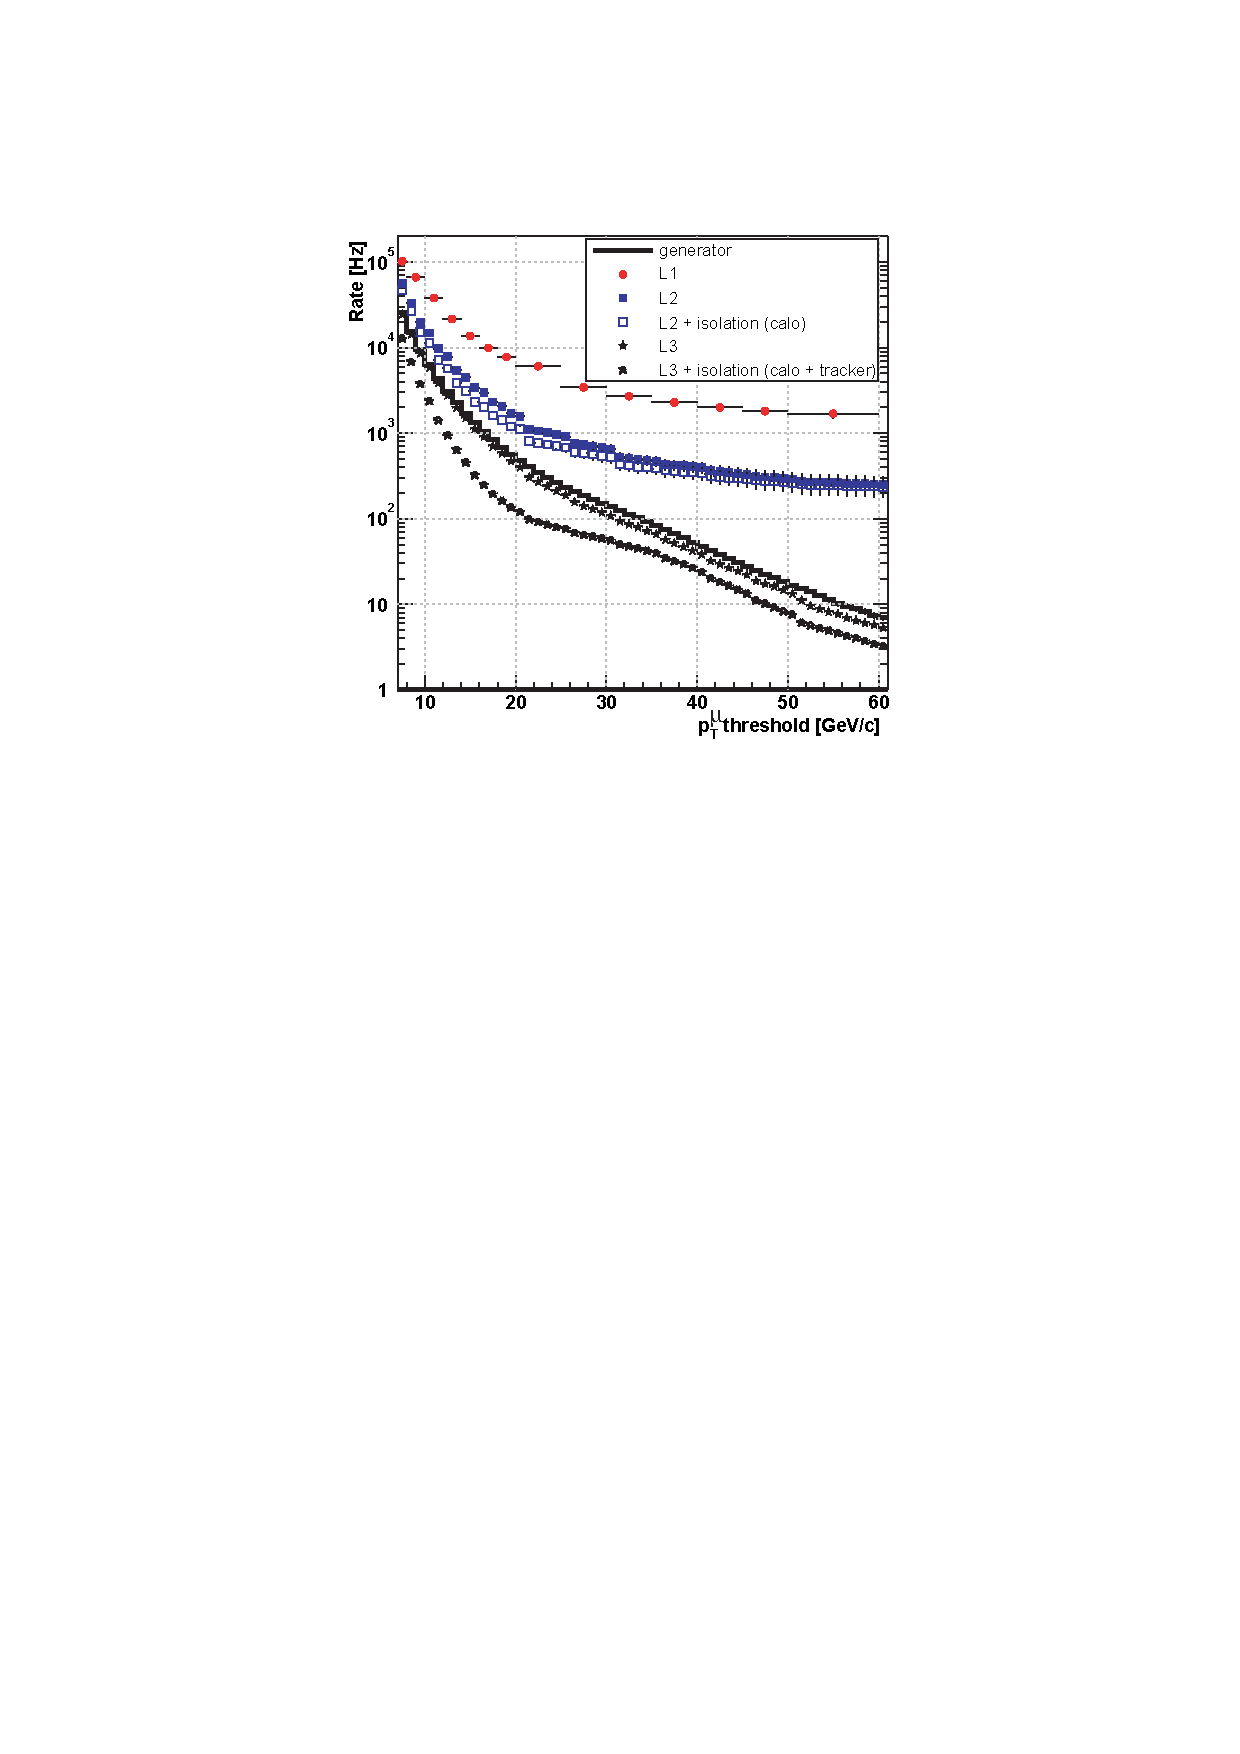
\includegraphics[width=0.5\textwidth]{Figures/pooth/pt_threshold.pdf}
\caption{Rates for different trigger levels as a function of the muon $p_t$ threshold~(REFREF).}
\label{fig:pt_threshold}
\end{figure}

This document is structured as follows:
\begin{itemize}
\item Prototype modules
	\begin{itemize}
	\item Silicon Photomultipliers and Frontend Electronics
	\item Measurements
	\item Simulations
	\end{itemize}
\item SiPM Upgrade in HO 
\item HO studies as an MTT testbed
\item MTT simulations in CMSSW
\item Ghost studies and interplay between MTT and existing CMS muon trigger
\end{itemize}

\end{document}  